\begin{figure}[htbp]
\centering
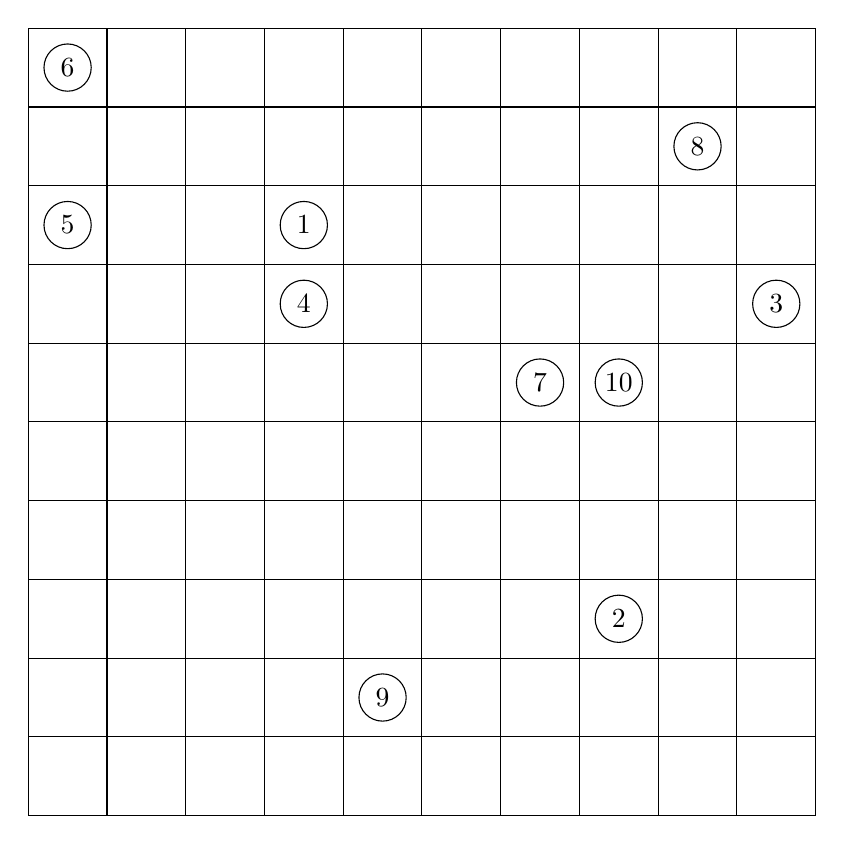
\begin{tikzpicture}

	\draw[xshift=0.5cm, yshift=0.5cm] (0,0) grid (10,10);
	\draw (4,8) circle [radius=0.3];
	\draw (8,3) circle [radius=0.3];
	\draw (10, 7) circle [radius=0.3];
	\draw (4, 7)  circle [radius=0.3];
	\draw (1, 8)  circle [radius=0.3];
	\draw (1, 10) circle [radius=0.3];
	\draw (7, 6)  circle [radius=0.3];
	\draw (9, 9)  circle [radius=0.3];
	\draw (5, 2)  circle [radius=0.3];
	\draw (8, 6)  circle [radius=0.3];

	\draw (4,8) node {1};
	\draw (8,3) node {2};
	\draw (10, 7) node{3};
	\draw (4, 7)  node{4};
	\draw (1, 8)  node{5};
	\draw (1, 10) node{6};
	\draw (7, 6)  node{7};
	\draw (9, 9)  node{8};
	\draw (5, 2)  node{9};
	\draw (8, 6)  node{10};
	
\end{tikzpicture}

\emph{Se tienen 4 centrales disponibles}

\caption{La entrada del problema, con las 10 ciudades y la cantidad de centrales}
\label{ej_2:aleatorio}
\end{figure}

